% Options for packages loaded elsewhere
\PassOptionsToPackage{unicode}{hyperref}
\PassOptionsToPackage{hyphens}{url}
\PassOptionsToPackage{dvipsnames,svgnames,x11names}{xcolor}
%
\documentclass[
  12pt,
  a4paper,
]{scrreprt}

\usepackage{amsmath,amssymb}
\usepackage{iftex}
\ifPDFTeX
  \usepackage[T1]{fontenc}
  \usepackage[utf8]{inputenc}
  \usepackage{textcomp} % provide euro and other symbols
\else % if luatex or xetex
  \usepackage{unicode-math}
  \defaultfontfeatures{Scale=MatchLowercase}
  \defaultfontfeatures[\rmfamily]{Ligatures=TeX,Scale=1}
\fi
\usepackage{lmodern}
\ifPDFTeX\else  
    % xetex/luatex font selection
\fi
% Use upquote if available, for straight quotes in verbatim environments
\IfFileExists{upquote.sty}{\usepackage{upquote}}{}
\IfFileExists{microtype.sty}{% use microtype if available
  \usepackage[]{microtype}
  \UseMicrotypeSet[protrusion]{basicmath} % disable protrusion for tt fonts
}{}
\usepackage{xcolor}
\usepackage[left=3cm,,right=2cm,,top=3cm,,bottom=2cm]{geometry}
\setlength{\emergencystretch}{3em} % prevent overfull lines
\setcounter{secnumdepth}{5}


\providecommand{\tightlist}{%
  \setlength{\itemsep}{0pt}\setlength{\parskip}{0pt}}\usepackage{longtable,booktabs,array}
\usepackage{calc} % for calculating minipage widths
% Correct order of tables after \paragraph or \subparagraph
\usepackage{etoolbox}
\makeatletter
\patchcmd\longtable{\par}{\if@noskipsec\mbox{}\fi\par}{}{}
\makeatother
% Allow footnotes in longtable head/foot
\IfFileExists{footnotehyper.sty}{\usepackage{footnotehyper}}{\usepackage{footnote}}
\makesavenoteenv{longtable}
\usepackage{graphicx}
\makeatletter
\newsavebox\pandoc@box
\newcommand*\pandocbounded[1]{% scales image to fit in text height/width
  \sbox\pandoc@box{#1}%
  \Gscale@div\@tempa{\textheight}{\dimexpr\ht\pandoc@box+\dp\pandoc@box\relax}%
  \Gscale@div\@tempb{\linewidth}{\wd\pandoc@box}%
  \ifdim\@tempb\p@<\@tempa\p@\let\@tempa\@tempb\fi% select the smaller of both
  \ifdim\@tempa\p@<\p@\scalebox{\@tempa}{\usebox\pandoc@box}%
  \else\usebox{\pandoc@box}%
  \fi%
}
% Set default figure placement to htbp
\def\fps@figure{htbp}
\makeatother

\usepackage{dirtree}
\usepackage{amsmath}
\usepackage[explicit]{titlesec}
\usepackage{setspace}
\usepackage{caption}
\usepackage[hang,flushmargin]{footmisc}
\usepackage{etoolbox}
\usepackage[shortlabels]{enumitem}
\usepackage{booktabs}
\usepackage{ragged2e}
\usepackage{pdflscape}
\usepackage{fancyhdr}

\newcommand{\blandscape}{\begin{landscape}}
\newcommand{\elandscape}{\end{landscape}}
\renewcommand{\footnotesize}{\scriptsize}
\renewcommand{\footnoterule}{\noindent\rule{5cm}{0.4pt}\vspace{0.2cm}}
\setlength{\footnotesep}{0.5em}

\setlength{\parskip}{0.0em}
\AtBeginEnvironment{quote}{\setstretch{1.0}}

\titleformat{\section}{\normalfont\large\bfseries}{}{0pt}{\thesection\quad#1}[]
\titleformat{\subsection}{\normalfont\normalsize\bfseries}{}{0pt}{\thesubsection\quad#1}[]
\titleformat{\subsubsection}{\normalfont\normalsize\itshape}{}{0pt}{#1}[]
\titleformat{\paragraph}[runin]{\normalfont\normalsize\bfseries}{}{0pt}{#1}[]
\titleformat{\subparagraph}[runin]{\normalfont\normalsize\itshape}{}{0pt}{#1}[]

\titlespacing*{\section}{0pt}{20pt}{10pt}
\titlespacing*{\subsection}{0pt}{15pt}{10pt}
\titlespacing*{\subsubsection}{0pt}{10pt}{10pt}
\titlespacing*{\paragraph}{0pt}{10pt}{10pt}
\titlespacing*{\subparagraph}{0pt}{10pt}{10pt}
\makeatletter
\@ifpackageloaded{caption}{}{\usepackage{caption}}
\AtBeginDocument{%
\ifdefined\contentsname
  \renewcommand*\contentsname{Índice}
\else
  \newcommand\contentsname{Índice}
\fi
\ifdefined\listfigurename
  \renewcommand*\listfigurename{Lista de Figuras}
\else
  \newcommand\listfigurename{Lista de Figuras}
\fi
\ifdefined\listtablename
  \renewcommand*\listtablename{Lista de Tabelas}
\else
  \newcommand\listtablename{Lista de Tabelas}
\fi
\ifdefined\figurename
  \renewcommand*\figurename{Figura}
\else
  \newcommand\figurename{Figura}
\fi
\ifdefined\tablename
  \renewcommand*\tablename{Tabela}
\else
  \newcommand\tablename{Tabela}
\fi
}
\@ifpackageloaded{float}{}{\usepackage{float}}
\floatstyle{ruled}
\@ifundefined{c@chapter}{\newfloat{codelisting}{h}{lop}}{\newfloat{codelisting}{h}{lop}[chapter]}
\floatname{codelisting}{Listagem}
\newcommand*\listoflistings{\listof{codelisting}{Lista de Listagens}}
\makeatother
\makeatletter
\makeatother
\makeatletter
\@ifpackageloaded{caption}{}{\usepackage{caption}}
\@ifpackageloaded{subcaption}{}{\usepackage{subcaption}}
\makeatother
\makeatletter
\@ifpackageloaded{tcolorbox}{}{\usepackage[skins,breakable]{tcolorbox}}
\makeatother
\makeatletter
\@ifundefined{shadecolor}{\definecolor{shadecolor}{rgb}{.97, .97, .97}}{}
\makeatother
\makeatletter
\@ifundefined{codebgcolor}{\definecolor{codebgcolor}{HTML}{F0F2F4}}{}
\makeatother
\makeatletter
\ifdefined\Shaded\renewenvironment{Shaded}{\begin{tcolorbox}[frame hidden, sharp corners, colback={codebgcolor}, boxrule=0pt, enhanced, breakable]}{\end{tcolorbox}}\fi
\makeatother

\ifLuaTeX
\usepackage[bidi=basic]{babel}
\else
\usepackage[bidi=default]{babel}
\fi
\babelprovide[main,import]{brazilian}
% get rid of language-specific shorthands (see #6817):
\let\LanguageShortHands\languageshorthands
\def\languageshorthands#1{}
\usepackage{bookmark}

\IfFileExists{xurl.sty}{\usepackage{xurl}}{} % add URL line breaks if available
\urlstyle{same} % disable monospaced font for URLs
\hypersetup{
  pdftitle={Segundo relatório da disciplina de demografia II - Roraima},
  pdfauthor={Gabriel de Jesus Pereira},
  pdflang={pt-br},
  colorlinks=true,
  linkcolor={blue},
  filecolor={Maroon},
  citecolor={Blue},
  urlcolor={Blue},
  pdfcreator={LaTeX via pandoc}}


\title{Segundo relatório da disciplina de demografia II - Roraima}
\author{Gabriel de Jesus Pereira}
\date{abril, 2025}

\begin{document}
\cleardoublepage
\thispagestyle{empty}
{\centering
\noindent\rule{\textwidth}{0.5pt}

\vspace{2ex}

{\Large\bfseries Universidade Federal da Paraíba \par}
\vspace{1ex}
{\Large\bfseries Centro de Ciências Exatas e da Natureza \par}
\vspace{1ex}
{\Large\bfseries Departamento de Estatística \par}

\vfill

{\large\bfseries Segundo relatório da disciplina de demografia II -
Roraima \par}

\vfill

{\large Gabriel de Jesus Pereira \par}
\vfill
{\normalsize abril, 2025 \par}


\noindent\rule{\textwidth}{0.5pt}

}
\renewcommand*\contentsname{\centering Sumário \thispagestyle{empty}}
{
\hypersetup{linkcolor=}
\setcounter{tocdepth}{2}
\tableofcontents
}

\pagenumbering{arabic}
\pagestyle{fancy}

\fancyhf{}
\fancyhead[RO, LE]{\thepage}
\fancyhead[LO]{\leftmark}
\fancyhead[RE]{\thepage}

\fancypagestyle{plain}{
  \pagestyle{fancy}
  \fancyhf{}
  \fancyhead[RO, LE]{\thepage}
  \fancyhead[RE]{\thepage}
  \renewcommand{\headrulewidth}{0pt}
}

\chapter{Introdução}\label{introduuxe7uxe3o}

\section{Recursos computacionais}\label{recursos-computacionais}

\chapter{Metodologia}\label{metodologia}

\section{Técnica de sobrevivência de
Brass}\label{tuxe9cnica-de-sobrevivuxeancia-de-brass}

A técnica de sobrevivência de Brass, proposta por William Brass, é um
método indireto utilizado para estimar níveis de mortalidade infantil e
na infância em populações com dados vitais incompletos ou de baixa
qualidade. O método baseia-se em informações obtidas a partir de censos
ou pesquisas domiciliares, onde as mulheres são questionadas sobre
número de filhos nascidos vivos e número de filhos sobreviventes na data
do censo por grupos de idade das mulheres, em diferentes faixas etárias
reprodutivas.

\vspace{12pt}

Para sua aplicação, o método de Brass pressupõe algumas características.
Por exemplo, A fecundidade específica por idade tem sido aproximadamente
constante no passado recente, coeficientes de mortalidade infantil e na
infância têm sido aproximadamente constantes, não há acentuada
associação entre mortalidade infantil e idade da mãe ou entre os
coeficientes de mortalidade das mães e dos seus filhos, taxas de
subenumeração para crianças sobreviventes e não sobreviventes são
aproximadamente iguais. Por último, O ``padrão etário'' de mortalidade
para idades jovens segue aproximadamente os padrões das tábuas-modelo

\vspace{12pt}

o princípio do método é que, conhecendo o número de filhos nascidos e o
número de filhos sobreviventes, é possível calcular a proporção de
filhos falecidos para cada grupo etário de mães. Essa proporção reflete
indiretamente o nível de mortalidade infantil, já que mulheres mais
velhas, por exemplo, tiveram filhos há mais tempo, e portanto o risco
acumulado de morte é maior entre seus filhos.

\vspace{12pt}

A fórmula básica usada é:

\[
D_i = 1 - \frac{\text{FV}_i}{\text{FNV}_i}\text{, }
\] em que \(\text{FV}_i\) é o número de filhos sobreviventes na data do
censo por grupos de idade das mulheres e \(\text{FNV}_i\) é o número de
nascidos vivos por grupo etário das mulheres.

\vspace{12pt}

Utilizando-se a relação entre a proporção de filhos mortos, \(D_i\), e a
probabilidade de morrer da tábua de vida, \(q_x\), Brass estabeleceu um
conjunto de multiplicadores, \(k_i\), que podem ser calculados a partir
de interpolação linear a partir da tabela padrão a seguir:

\begin{figure}[H]

{\centering \pandocbounded{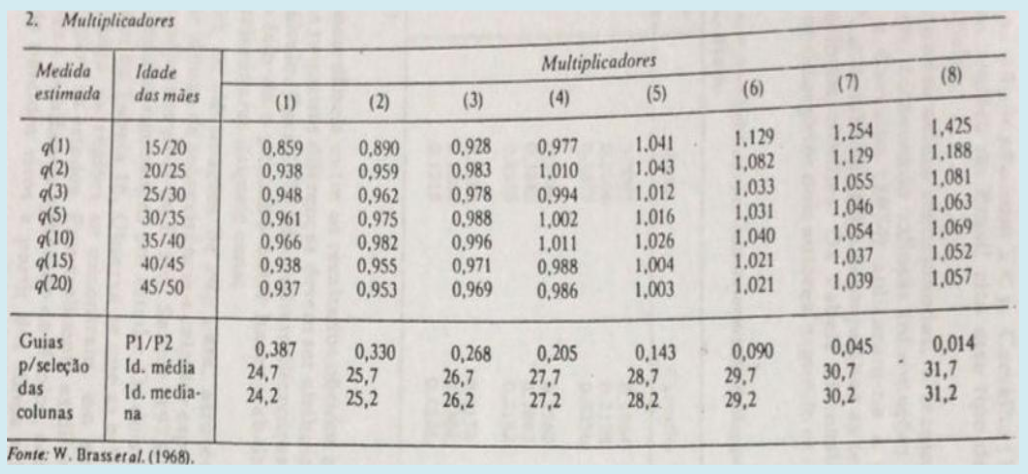
\includegraphics[keepaspectratio]{includes/sob_brass.png}}

}

\caption{Tabela para determinação de multiplicadores \(k_i\).}

\end{figure}%

Agora, com esses valores \(k_i\), pode-se converter os valores
observados \(D_i\) em estimativas de \(q_x\), ou seja, probabilidade de
morte entre o nascimento e idades exatas:

\[
q_x = k_i D_i\text{.}
\]

Tendo estimado o conjunto de probabilidades de morte \(q_x\), obtém-se,
por diferença, a probabilidade de sobrevivência entre o nascimento e
idades exatas, \(I_x\):

\[
I_x = I - q_x\text{.}
\]

\section{Técnica de Brass para estimar a
fecundidade}\label{tuxe9cnica-de-brass-para-estimar-a-fecundidade}

~~~O objetivo da técnica de Brass estimar a fecundidade é estimar a
fecundidade em países cujos dados de registro civil não permitem um
cálculo razoável do seu nível.

\vspace{12pt}

Um de seus pressupostos parar aplicação do método é que a fecundidade
tenha sido aproximadamente constante no passado recente. Além desse
pressuposto, é necessário também que os coeficientes específicos de
fecundidade por idade da mulher, tais como os obtidos através de
perguntas diretas, são corretos quanto ao padrão etário da fecundidade e
o nível de fecundidade é corretamente medido através do número de filhos
tidos (nascidos vivos) informados pelas mulheres mais jovens (usualmente
do grupo etário 20-25) -- ou seja, através da parturição média dessas
mulheres.

\vspace{12pt}

Para utilizar a técnica de Brass, será necessário calcular os nascidos
vivos no ano anterior ao censo por mulher, que é denotado por \(f_i\),
total de nascidos vivos por mulher \(P_i\). A partir de \(f_i\),
calcula-se a fucundidade acumulada no começo do intervalo
\(F^{'}_i = 5 \sum_{j=0}^{i-1} f_{j}\). Uma das outras componentes que
compõe o método são os fatores de multiplicação \(W_i\), que são valores
tabelados e que podem ser calculados por interporlação linear a partir
do intervalo que \(f_{1}/f_{2}\) estão definidos na tabela a seguir:

\begin{figure}[H]

{\centering \pandocbounded{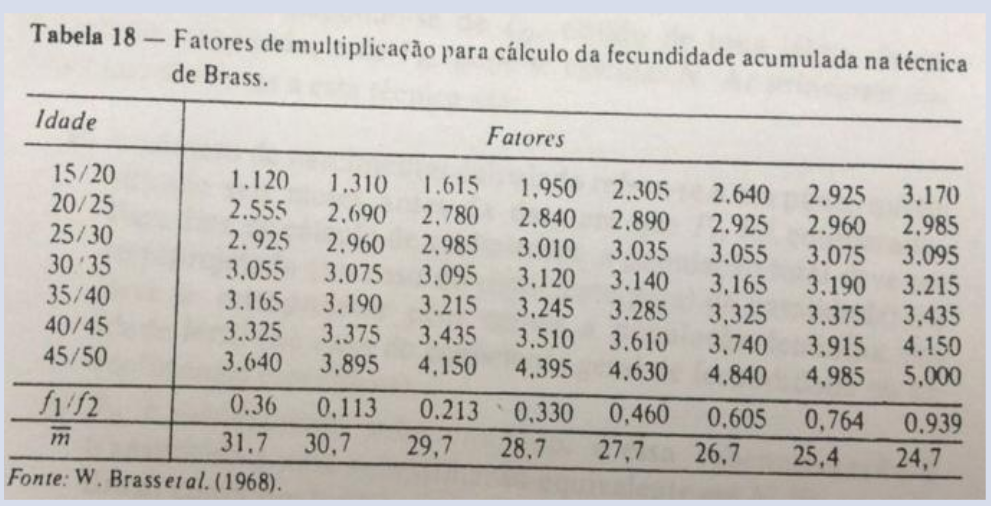
\includegraphics[keepaspectratio]{includes/fatores_mult.png}}

}

\caption{Valores tabelados para cálculo de fatores de multiplicação
\(W_i\).}

\end{figure}%

Após encontrar os fatores de multiplicação \(W_i\), basta cálcular a
fecundidade acumulada média com \(F_i =  F_i + W_if_i\). Por fim,
encontram-se os coeficientes específicos corrigidos
\(f^{'}=f_iP_{2}/F_{2}\).

\section{Modelando taxa de fecundidade
marital}\label{modelando-taxa-de-fecundidade-marital}

~~~O modelo de fecundidade marital de Coale-Trussell é uma das
abordagens clássicas para estudar o comportamento reprodutivo de
mulheres casadas, oferecendo uma maneira prática de estimar e
interpretar padrões de fecundidade observados com base em uma
curva-padrão e parâmetros de ajuste. Sua aplicação é especialmente útil
em estudos demográficos comparativos entre diferentes regiões ou ao
longo do tempo.

\vspace{12pt}

O modelo parte da ideia de que a fecundidade marital observada pode ser
representada como uma modificação de um padrão considerado ``natural''
ou ``biológico'' de fecundidade. A fórmula principal é:

\[
f\left(a\right) = G\left(a\right) r\left(a\right)\text{, }
\] em que \(a\) é a idade, \(f\left(a\right)\) é a taxa específica de
fecundidade, \(G\left(a\right)\) é o risco do primeiro casamento,
\(r\left(a\right)\) é a taxa específica de fecundidade marital, a qual é
expressa da seguinte forma:

\[
r\left(a\right) = M n\left(a\right) e^{m v\left(a\right)} \text{, }
\] em que \(M\) é o nível de fecundidade e \(m\) é o padrão de
fecundidade. \(n\left(a\right)\) é a fecundidade marital natural e
\(v\left(a\right)\) é a fecundidade fixa.

\vspace{12pt}

Por fim, a partir da expressão de \(r\left(a\right)\) pode ser definida
uma regressão linear da seguinte forma:

\[
\ln\left(r\left(a\right) / n\left(a\right)\right) = \ln\left(M\right) + mv\left(a\right)
\]

\vspace{12pt}

Além disso, vale ressaltar que a fecundidade marital e natural e a
fecundidade fixa são derivadas por experiência de alguns países,
principalmente europeus. A imagem a seguir mostra os valores que foram
considerados para esse trabalho:

\begin{figure}[H]

{\centering \pandocbounded{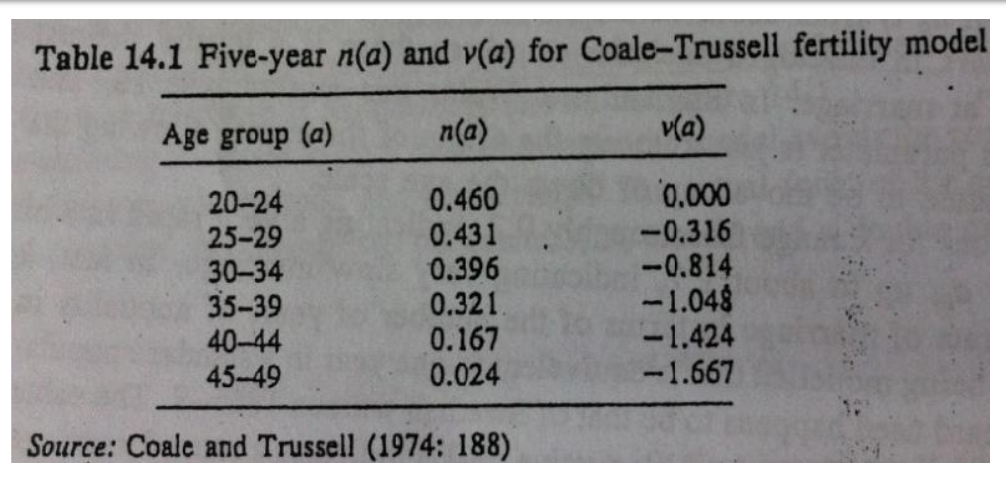
\includegraphics[keepaspectratio]{includes/tabela_coell.png}}

}

\caption{Valores tabelados de \(n\left(a\right)\) e \(v\left(a\right)\)
para aplicação do método de Coale-Trussel.}

\end{figure}%

\section{Modelo relacional de
Gompertz}\label{modelo-relacional-de-gompertz}

~~~O modelo relacional de Gompertz é uma metodologia demográfica
amplamente utilizada para descrever e ajustar padrões de fecundidade,
especialmente quando os dados observados apresentam problemas de
cobertura ou qualidade. Sua principal utilidade está em permitir
comparações entre diferentes populações ou períodos por meio de uma
curva-padrão acumulada de fecundidade.

\vspace{12pt}

A lógica do modelo baseia-se na função de Gompertz, originalmente
utilizada para modelar taxas de mortalidade, mas que também pode ser
aplicada ao padrão acumulado da fecundidade, \(F\left(a\right)\), isto
é, a proporção da fecundidade total que já ocorreu até determinada idade
\(a\). O modelo assume a seguinte forma funcional:

\[
\text{Gompit}\left(F\left(a\right)\right) = \ln\left[-\ln\left(1-F\left(a\right)\right)\right] = \alpha + \beta\text{Gompit}\left(F_{s}\left(a\right)\right)
\] em que \(F\left(a\right)\) é a distribuição acumulada de fecundidade
da população observada, \(F_{s}\left(a\right)\) é a distribuição
acumulada de fecundidade da população padrão, \(-0,5< \alpha < 0,5\) e
\(0,65 < \beta < 1,5\) são o nível da fecundidade e padrão da
fecundidade, respectivamente.

\vspace{12pt}

Para aplicar o modelo, é necessário calcular a distribuição proporcional
das taxas específicas de fecundidade \(p\left(a\right)\), obter a
distribuição acumulada \(F\left(a\right)\), aplicar a transformação
Gompit \(\ln\left[-\ln\left(1 - F\left(a\right)\right)\right]\), ajustar
uma regressão linear entre os gompits da população observada e os da
curva padrão e, por fim, estimar os parâmetros \(\alpha\) e \(\beta\),
que permitem reconstruir a curva ajustada ou fazer comparações com
outras populações.

\chapter{Resultados}\label{resultados}

\section{Técnica de sobrevivência de
Brass}\label{tuxe9cnica-de-sobrevivuxeancia-de-brass-1}

\blandscape

\section{Técnica de Brass para a
fecundidade}\label{tuxe9cnica-de-brass-para-a-fecundidade}

~~~Na faixa de 20 a 24 anos, a fecundidade começa a aumentar, com uma
taxa de fecundidade corrigida de 0,918372 e um valor acumulado
(fi\_acum) de 2,950542. Isso reflete um aumento na fecundidade, que
geralmente ocorre à medida que as mulheres atingem idades mais próximas
do pico reprodutivo. O valor de 0,065290 para o ajuste de fecundidade
também está dentro do esperado, indicando que a técnica Brass está
corrigindo adequadamente os dados.

\vspace{12pt}

Nas faixas de 25 a 29 anos e 30 a 34 anos, a fecundidade continua a
aumentar, atingindo valores de fi corrigido de 1,518141 e 1,937938,
respectivamente, com valores de fi acumulado chegando a 3,069595 e
3,183244. Isso é consistente com a expectativa, pois a fecundidade
atinge seu pico em torno de 30 anos, e as mulheres dessa faixa etária
tendem a ter mais filhos.

\vspace{12pt}

Finalmente, na faixa de 45 a 49 anos, a fecundidade é muito baixa, como
esperado para essa faixa etária. O valor de fi corrigido de 2,322042 é
alto em relação ao número de nascimentos (1,610,379), refletindo a
diminuição significativa na fecundidade após os 40 anos. A técnica de
Brass consegue corrigir adequadamente os dados, gerando uma taxa de
fecundidade realista para as mulheres dessa faixa etária avançada.

\(0.096731 / 0.134156 = 0.721033721935657\)

\((0.764 - 0.721033721935657) / (0.764 - 0.605) = 0.2702281639266858\)

\begin{longtable}[]{@{}llllllllll@{}}
\caption{}\label{T_fee00}\tabularnewline
\toprule\noalign{}
Idade & Nascidos & Mulheres & Nascidos\_vivos\_2009 & fi & Pi & Fi & Wi
& Fi\_acum\_media & fi\_corrigido \\
\midrule\noalign{}
\endfirsthead
\toprule\noalign{}
Idade & Nascidos & Mulheres & Nascidos\_vivos\_2009 & fi & Pi & Fi & Wi
& Fi\_acum\_media & fi\_corrigido \\
\midrule\noalign{}
\endhead
\bottomrule\noalign{}
\endlastfoot
15 a 19 anos & 2253 & 23250 & 2249 & 0.096731 & 0.418839 & 0.038882 &
2.847985 & 0.314371 & 0.047076 \\
20 a 24 anos & 2866 & 21788 & 2923 & 0.134156 & 0.446943 & 0.522538 &
2.950542 & 0.918372 & 0.065290 \\
25 a 29 anos & 2276 & 21792 & 2306 & 0.105819 & 0.446861 & 1.193320 &
3.069595 & 1.518141 & 0.051499 \\
30 a 34 anos & 1394 & 18669 & 1264 & 0.067706 & 0.521613 & 1.722414 &
3.183244 & 1.937938 & 0.032950 \\
35 a 39 anos & 587 & 14839 & 542 & 0.036525 & 0.656244 & 2.060943 &
3.361489 & 2.183722 & 0.017776 \\
40 a 44 anos & 155 & 12269 & 168 & 0.013693 & 0.793708 & 2.243570 &
3.867710 & 2.296530 & 0.006664 \\
45 a 49 anos & 16 & 10379 & 21 & 0.002023 & 0.938241 & 2.312035 &
4.945817 & 2.322042 & 0.000985 \\
\end{longtable}

\elandscape

\blandscape

\section{Modelando taxa de fecundidade
marital}\label{modelando-taxa-de-fecundidade-marital-1}

~~~Na faixa de 20 a 24 anos, a fecundidade marital observada (0.053424)
está próxima da estimada (0.062416), o que indica que o modelo consegue
capturar bem a dinâmica reprodutiva das mulheres casadas nesse grupo.
Conforme a idade avança, como na faixa de 25 a 29 anos, a fecundidade
observada diminui levemente (0.053185), mas o modelo ainda mantém boa
aderência ao produzir um valor estimado compatível (0.048705). Na faixa
de 30 a 34 anos, a queda na fecundidade é mais acentuada (0.043441), e
novamente o modelo responde de forma adequada, com valor estimado de
0.033542, demonstrando sensibilidade ao declínio na intensidade
reprodutiva. Esse padrão se mantém nas idades seguintes: de 35 a 39
anos, há um recuo substancial na fecundidade (0.022913), e o valor
ajustado (0.023745) reflete com precisão essa mudança

\begin{longtable}[]{@{}lllllllll@{}}
\caption{}\label{T_9e95a}\tabularnewline
\toprule\noalign{}
Idade & TFE & v\_a & n\_a & Mulheres & Nascimentos\_casadas & r\_a &
log\_r\_a\_n\_a & r\_a\_estimado \\
\midrule\noalign{}
\endfirsthead
\toprule\noalign{}
Idade & TFE & v\_a & n\_a & Mulheres & Nascimentos\_casadas & r\_a &
log\_r\_a\_n\_a & r\_a\_estimado \\
\midrule\noalign{}
\endhead
\bottomrule\noalign{}
\endlastfoot
20 a 24 anos & 0.150450 & 0.000000 & 0.460000 & 21788 & 1164 & 0.053424
& -2.152968 & 0.062416 \\
25 a 29 anos & 0.121020 & -0.316000 & 0.431000 & 21792 & 1159 & 0.053185
& -2.092338 & 0.048705 \\
30 a 34 anos & 0.081270 & -0.814000 & 0.396000 & 18669 & 811 & 0.043441
& -2.210011 & 0.033542 \\
35 a 39 anos & 0.044710 & -1.048000 & 0.321000 & 14839 & 340 & 0.022913
& -2.639754 & 0.023745 \\
40 a 44 anos & 0.014680 & -1.424000 & 0.167000 & 12269 & 96 & 0.007825 &
-3.060721 & 0.009937 \\
45 a 49 anos & 0.001680 & -1.667000 & 0.024000 & 10379 & 14 & 0.001349 &
-2.878781 & 0.001241 \\
\end{longtable}

\elandscape

\blandscape

\section{Modelo relacional de
Gompertz}\label{modelo-relacional-de-gompertz-1}

~~~Na faixa de 15 a 19 anos, os valores de \(f\left(a\right)\) e
\(f′\left(a\right)\) indicam que o modelo superestima um pouco a
fecundidade específica (0.220 vs 0.137 observada), ainda que a acumulada
p′(a)p′(a) esteja razoavelmente próxima. Isso pode ser reflexo de um
início mais precoce da fecundidade do que o padrão esperado.

\vspace{12pt}

Entre 20 e 24 anos, o modelo começa a se ajustar melhor, com
\(f^{'}\left(a\right)=0.1519\) sendo mais próximo de \(F_a=0.1504\), e o
valor acumulado \(p^{'}(a)\approx 0.51\), em linha com a acumulação
observada. Isso sugere que o modelo consegue captar bem a intensidade e
a forma da fecundidade nesse pico inicial.

\vspace{12pt}

De 25 a 29 anos, o modelo continua a fornecer uma boa aproximação tanto
para a fecundidade específica quanto para a acumulada, o que indica que
ele ajusta corretamente o pico de fecundidade típico dessa faixa etária,
que é o período de maior concentração de nascimentos.

\vspace{12pt}

Nas faixas de 35 a 39 e 40 a 44 anos, o modelo ajusta valores muito
baixos de \(f^{'}(a)\), o que é esperado, pois essas idades correspondem
ao final do período reprodutivo. O ajuste segue a tendência esperada de
declínio acentuado, com valores próximos a zero, sem gerar disrupções
artificiais.

\begin{longtable}[]{@{}llllllllllll@{}}
\caption{}\label{T_9c8c4}\tabularnewline
\toprule\noalign{}
Idade & TFE & p\_a & idade\_e & F\_a & G & F\_a\_padrao & G\_padrao &
G\textquotesingle{} & antgompt & p\textquotesingle(a) &
f\textquotesingle(a) \\
\midrule\noalign{}
\endfirsthead
\toprule\noalign{}
Idade & TFE & p\_a & idade\_e & F\_a & G & F\_a\_padrao & G\_padrao &
G\textquotesingle{} & antgompt & p\textquotesingle(a) &
f\textquotesingle(a) \\
\midrule\noalign{}
\endhead
\bottomrule\noalign{}
\endlastfoot
15 a 19 anos & 0.110630 & 0.210949 & 20 & 0.210949 & -0.442208 &
0.136000 & -0.691000 & -0.414074 & 0.220255 & 4.540190 & 2.373430 \\
20 a 24 anos & 0.150450 & 0.286877 & 25 & 0.497826 & 0.360247 & 0.377000
& 0.026000 & 0.398204 & 0.510929 & 0.290674 & 0.151953 \\
25 a 29 anos & 0.121020 & 0.230760 & 30 & 0.728587 & 1.149962 & 0.609000
& 0.700000 & 1.161767 & 0.731299 & 0.220370 & 0.115201 \\
30 a 34 anos & 0.081270 & 0.154965 & 35 & 0.883552 & 2.089046 & 0.796000
& 1.479000 & 2.044284 & 0.878558 & 0.147259 & 0.076981 \\
35 a 39 anos & 0.044710 & 0.085253 & 40 & 0.968805 & 3.451687 & 0.930000
& 2.626000 & 3.343701 & 0.965310 & 0.086752 & 0.045350 \\
40 a 44 anos & 0.014680 & 0.027992 & 45 & 0.996797 & 5.741933 & 0.992000
& 4.809000 & 5.816786 & 0.997027 & 0.031717 & 0.016581 \\
\end{longtable}

\elandscape

\chapter{Exercícios do Mortpak}\label{exercuxedcios-do-mortpak}

\begin{figure}

\begin{minipage}{\linewidth}

\begin{figure}[H]

\centering{

\pandocbounded{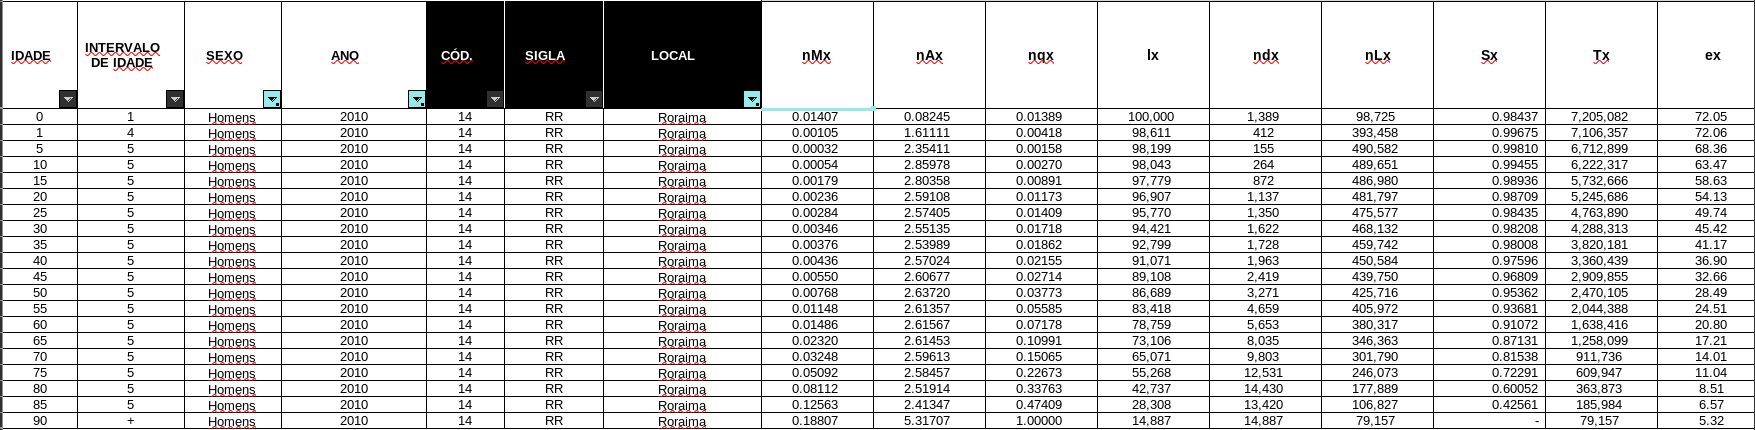
\includegraphics[keepaspectratio]{includes/tabua_vida_homens.png}}

}

\caption{\label{fig-tabua_vida_masc}Tábua de vida para o sexo
masculino.}

\end{figure}%

\end{minipage}%
\newline
\begin{minipage}{\linewidth}

\begin{figure}[H]

\centering{

\pandocbounded{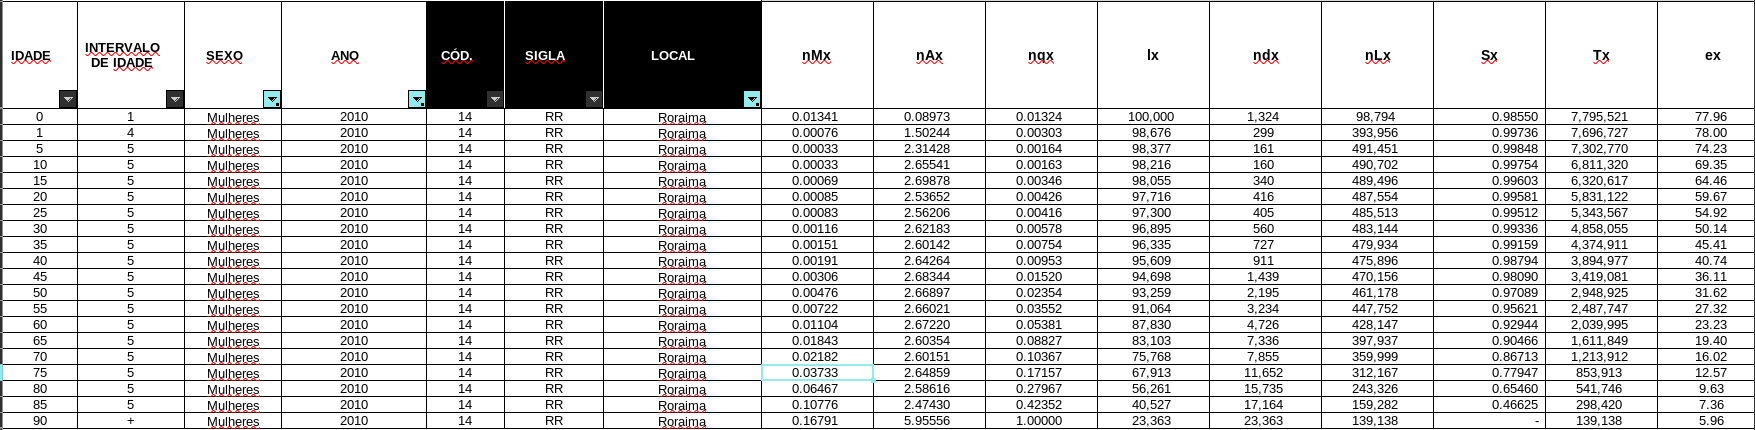
\includegraphics[keepaspectratio]{includes/tabua_vida_mulheres.png}}

}

\caption{\label{fig-tabua_vida_fem}Tábua de vida para o sexo feminino.}

\end{figure}%

\end{minipage}%

\end{figure}%

\section{Questão 1)}\label{questuxe3o-1}

Ver no Mortpak qual é o melhor modelo ao comparar os Modelos das Nações
Unidas aos de Coale-Demeny (Função COMPAR);

\vspace{12pt}

Ao comparar os modelos das Nações Unidas com os de Coale-Demeny e
observar a expectativa de vida estimada para o sexo masculino na
Figura~\ref{fig-tabua_vida_masc}, nota-se que o modelo que mais se
aproxima é o Far East, das Nações Unidas. Por outro lado, no caso do
sexo feminino, o modelo que mais se aproxima é o East, de Coale-Demeny.

\begin{figure}

\begin{minipage}{0.50\linewidth}

\begin{figure}[H]

{\centering \pandocbounded{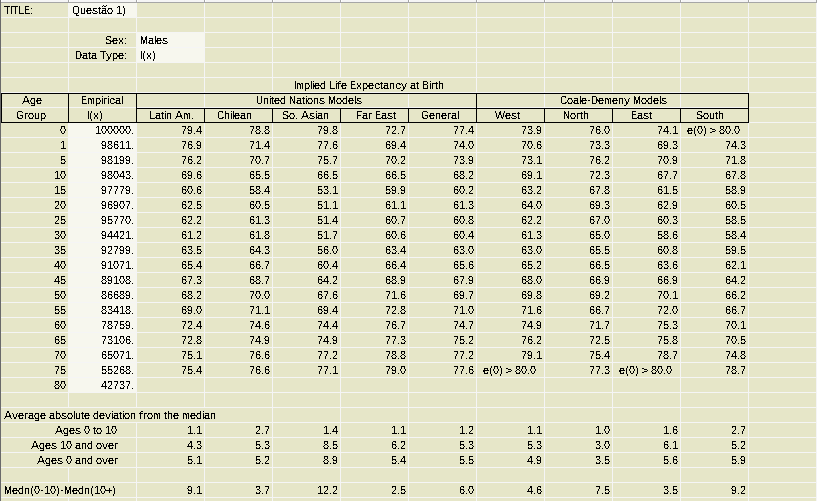
\includegraphics[keepaspectratio]{includes/expec_vida_homens.png}}

}

\subcaption{Função COMPAR para o sexo masculino.}

\end{figure}%

\end{minipage}%
%
\begin{minipage}{0.50\linewidth}

\begin{figure}[H]

{\centering \pandocbounded{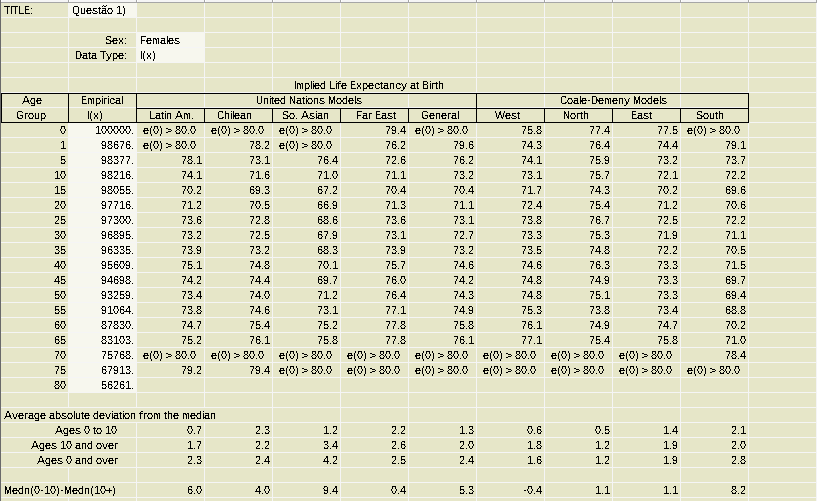
\includegraphics[keepaspectratio]{includes/expec_vida_mulheres.png}}

}

\subcaption{Função COMPAR para o sexo feminino.}

\end{figure}%

\end{minipage}%

\end{figure}%

\section{Questão 2)}\label{questuxe3o-2}

Considerar apenas os Modelos das Nações Unidas e ver qual é o melhor
(Função COMPAR);

\vspace{12pt}

O melhor modelo das Nações Unidas para o sexo masculino foi o de Far
East. Da mesma forma, o melhor modelo foi o de Far East.

\section{Questão 3)}\label{questuxe3o-3}

Observar os valores da \(E\left(x\right)\) e escolher a TV Modelo das
Nações Unidas mais adequada (depende do passo 2\ldots);

\section{Questão 4)}\label{questuxe3o-4}

Usar o sistema logito de tábuas de vida de dois parâmetros de Brass e
considerar os seguintes padrões: Modelo Geral de Brass; MAB e o
resultado do passo 3.

\subsection{Caso com o Modelo Geral de Brass
Homens}\label{caso-com-o-modelo-geral-de-brass-homens}

~~~Observa-se que, para as idades iniciais, os valores de I(x) estão
próximos de 1, indicando alta sobrevivência na infância, como esperado.
À medida que a idade avança, os valores de I(x) diminuem, refletindo o
aumento da mortalidade com o tempo. No entanto, ao comparar I(x) com
I(x) estimado GB, nota-se que o modelo tende a subestimar a
sobrevivência em praticamente todas as idades, ou seja, o valor ajustado
pelo modelo é sistematicamente inferior ao valor observado. Essa
diferença se torna mais evidente nas idades adultas e avançadas. Por
exemplo, aos 40 anos, o valor observado de I(x) é 0,911, enquanto o
estimado é 0,510, uma discrepância considerável. Isso sugere que a
população masculina analisada apresenta níveis de sobrevivência mais
altos do que os previstos pela tabela-padrão utilizada pelo modelo de
Brass.

\begin{longtable}[]{@{}lllllll@{}}
\caption{}\label{T_dd803}\tabularnewline
\toprule\noalign{}
Idade & I(x) & I(x) GB & Ys(x) & Y(x) & Y(x) estimado GB & I(x) estimado
GB \\
\midrule\noalign{}
\endfirsthead
\toprule\noalign{}
Idade & I(x) & I(x) GB & Ys(x) & Y(x) & Y(x) estimado GB & I(x) estimado
GB \\
\midrule\noalign{}
\endhead
\bottomrule\noalign{}
\endlastfoot
1,000 & 0,986 & 0,850 & -0,867 & -2,131 & -0,966 & 0,874 \\
5,000 & 0,982 & 0,769 & -0,602 & -1,999 & -0,838 & 0,842 \\
10,000 & 0,980 & 0,750 & -0,550 & -1,957 & -0,796 & 0,831 \\
15,000 & 0,978 & 0,736 & -0,513 & -1,892 & -0,733 & 0,813 \\
20,000 & 0,969 & 0,713 & -0,455 & -1,722 & -0,567 & 0,757 \\
25,000 & 0,958 & 0,683 & -0,383 & -1,560 & -0,409 & 0,694 \\
30,000 & 0,944 & 0,652 & -0,315 & -1,414 & -0,267 & 0,630 \\
35,000 & 0,928 & 0,622 & -0,250 & -1,278 & -0,134 & 0,567 \\
40,000 & 0,911 & 0,509 & -0,018 & -1,161 & -0,020 & 0,510 \\
45,000 & 0,891 & 0,553 & -0,107 & -1,051 & 0,088 & 0,456 \\
50,000 & 0,867 & 0,511 & -0,021 & -0,937 & 0,199 & 0,402 \\
55,000 & 0,834 & 0,459 & 0,082 & -0,808 & 0,325 & 0,343 \\
60,000 & 0,788 & 0,397 & 0,210 & -0,655 & 0,474 & 0,279 \\
65,000 & 0,731 & 0,322 & 0,372 & -0,500 & 0,626 & 0,223 \\
70,000 & 0,651 & 0,238 & 0,582 & -0,311 & 0,810 & 0,165 \\
75,000 & 0,553 & 0,152 & 0,859 & -0,106 & 1,010 & 0,117 \\
80,000 & 0,427 & 0,078 & 1,238 & 0,146 & 1,256 & 0,075 \\
85,000 & 0,283 & 0,028 & 1,772 & 0,465 & 1,567 & 0,042 \\
90,000 & 0,149 & 0,006 & 2,555 & 0,872 & 1,964 & 0,019 \\
\end{longtable}

\subsection{Caso com o MAB Homens}\label{caso-com-o-mab-homens}

~~~Aos 1 ano de idade, o valor observado de sobrevivência
\(I\left(x\right)\) é 0,986, enquanto o estimado pelo modelo é 0,862.
Apesar de uma leve subestimação, o valor já se aproxima bastante,
mostrando que o modelo é capaz de capturar adequadamente a alta
sobrevivência nos primeiros anos de vida, mesmo considerando a maior
mortalidade infantil masculina em comparação ao sexo feminino.

\vspace{12pt}

Ao longo da infância e juventude (até os 20--25 anos), o modelo continua
apresentando valores estimados que acompanham a tendência dos valores
observados, com pequenas diferenças --- o que indica bom ajuste. Por
exemplo, aos 25 anos, o \(I\left(x\right)\) observado é 0,958 e o
estimado é 0,704, o que representa uma redução coerente, considerando o
padrão de aumento de mortalidade nessa fase.

\begin{longtable}[]{@{}lllllll@{}}
\caption{}\label{T_4ad54}\tabularnewline
\toprule\noalign{}
Idade & I(x) & I(x) MAB & Ys(x) & Y(x) & Y(x) estimado MAB & I(x)
estimado MAB \\
\midrule\noalign{}
\endfirsthead
\toprule\noalign{}
Idade & I(x) & I(x) MAB & Ys(x) & Y(x) & Y(x) estimado MAB & I(x)
estimado MAB \\
\midrule\noalign{}
\endhead
\bottomrule\noalign{}
\endlastfoot
1,000 & 0,986 & 0,842 & -0,836 & -2,131 & -0,916 & 0,862 \\
5,000 & 0,982 & 0,759 & -0,574 & -1,999 & -0,804 & 0,833 \\
10,000 & 0,980 & 0,751 & -0,552 & -1,957 & -0,768 & 0,823 \\
15,000 & 0,978 & 0,745 & -0,536 & -1,892 & -0,714 & 0,807 \\
20,000 & 0,969 & 0,734 & -0,508 & -1,722 & -0,570 & 0,758 \\
25,000 & 0,958 & 0,717 & -0,465 & -1,560 & -0,433 & 0,704 \\
30,000 & 0,944 & 0,694 & -0,410 & -1,414 & -0,310 & 0,650 \\
35,000 & 0,928 & 0,664 & -0,341 & -1,278 & -0,194 & 0,596 \\
40,000 & 0,911 & 0,627 & -0,259 & -1,161 & -0,095 & 0,548 \\
45,000 & 0,891 & 0,585 & -0,172 & -1,051 & -0,002 & 0,501 \\
50,000 & 0,867 & 0,536 & -0,073 & -0,937 & 0,094 & 0,453 \\
55,000 & 0,834 & 0,487 & 0,027 & -0,808 & 0,203 & 0,400 \\
60,000 & 0,788 & 0,423 & 0,154 & -0,655 & 0,332 & 0,340 \\
65,000 & 0,731 & 0,347 & 0,317 & -0,500 & 0,464 & 0,283 \\
70,000 & 0,651 & 0,260 & 0,524 & -0,311 & 0,623 & 0,223 \\
75,000 & 0,553 & 0,167 & 0,804 & -0,106 & 0,797 & 0,169 \\
80,000 & 0,427 & 0,086 & 1,182 & 0,146 & 1,010 & 0,117 \\
85,000 & 0,283 & 0,031 & 1,716 & 0,465 & 1,279 & 0,072 \\
\end{longtable}

\subsection{Caso com o Modelo Geral de Brass
Mulheres}\label{caso-com-o-modelo-geral-de-brass-mulheres}

Nas idades avançadas, a sobrevivência observada das mulheres continua
sistematicamente superior aos valores estimados pelo modelo, como
evidencia, por exemplo, a idade de 60 anos, em que \(I\left(x\right)\) é
0,878 e \(I\left(x\right)\) estimado GB é 0,306, uma diferença
acentuada. Essa tendência se intensifica com o avanço da idade,
revelando que a tabela-padrão subestima a longevidade feminina na
população analisada. Isso está de acordo com o que se conhece
demograficamente: as mulheres têm maior expectativa de vida e sobrevivem
em maiores proporções nas idades avançadas em comparação aos homens.

\begin{longtable}[]{@{}lllllll@{}}
\caption{}\label{T_a282c}\tabularnewline
\toprule\noalign{}
Idade & I(x) & I(x) GB & Ys(x) & Y(x) & Y(x) estimado GB & I(x) estimado
GB \\
\midrule\noalign{}
\endfirsthead
\toprule\noalign{}
Idade & I(x) & I(x) GB & Ys(x) & Y(x) & Y(x) estimado GB & I(x) estimado
GB \\
\midrule\noalign{}
\endhead
\bottomrule\noalign{}
\endlastfoot
1,000 & 0,987 & 0,850 & -0,867 & -2,156 & -0,830 & 0,840 \\
5,000 & 0,984 & 0,769 & -0,602 & -2,052 & -0,720 & 0,809 \\
10,000 & 0,982 & 0,750 & -0,550 & -2,004 & -0,669 & 0,792 \\
15,000 & 0,981 & 0,736 & -0,513 & -1,960 & -0,622 & 0,776 \\
20,000 & 0,977 & 0,713 & -0,455 & -1,878 & -0,535 & 0,745 \\
25,000 & 0,973 & 0,683 & -0,383 & -1,792 & -0,444 & 0,709 \\
30,000 & 0,969 & 0,652 & -0,315 & -1,720 & -0,368 & 0,676 \\
35,000 & 0,963 & 0,622 & -0,250 & -1,635 & -0,277 & 0,635 \\
40,000 & 0,956 & 0,509 & -0,018 & -1,540 & -0,177 & 0,587 \\
45,000 & 0,947 & 0,553 & -0,107 & -1,441 & -0,072 & 0,536 \\
50,000 & 0,933 & 0,511 & -0,021 & -1,314 & 0,064 & 0,468 \\
55,000 & 0,911 & 0,459 & 0,082 & -1,161 & 0,226 & 0,389 \\
60,000 & 0,878 & 0,397 & 0,210 & -0,988 & 0,409 & 0,306 \\
65,000 & 0,831 & 0,322 & 0,372 & -0,796 & 0,613 & 0,227 \\
70,000 & 0,758 & 0,238 & 0,582 & -0,570 & 0,854 & 0,154 \\
75,000 & 0,679 & 0,152 & 0,859 & -0,375 & 1,061 & 0,107 \\
80,000 & 0,563 & 0,078 & 1,238 & -0,126 & 1,325 & 0,066 \\
85,000 & 0,405 & 0,028 & 1,772 & 0,192 & 1,662 & 0,035 \\
90,000 & 0,234 & 0,006 & 2,555 & 0,594 & 2,089 & 0,015 \\
\end{longtable}

\subsection{Caso com o MAB Mulheres}\label{caso-com-o-mab-mulheres}

~~~À medida que a idade avança, especialmente a partir dos 20 ou 25
anos, essa diferença entre os valores observados e estimados começa a
crescer. Ainda que o modelo continue refletindo a diminuição progressiva
da sobrevivência com a idade --- o que está em conformidade com a
realidade demográfica ---, ele tende a acentuar essa queda de forma um
pouco mais intensa do que a observada nos dados. Por exemplo, aos 40 e
50 anos, os valores de I(x)I(x) estimados já se distanciam mais
significativamente dos observados, o que pode indicar que o modelo
suaviza ou generaliza padrões que não capturam totalmente a dinâmica
real da mortalidade feminina brasileira nessas idades.

\begin{longtable}[]{@{}lllllll@{}}
\caption{}\label{T_b203a}\tabularnewline
\toprule\noalign{}
Idade & I(x) & I(x) MAB & Ys(x) & Y(x) & Y(x) estimado MAB & I(x)
estimado MAB \\
\midrule\noalign{}
\endfirsthead
\toprule\noalign{}
Idade & I(x) & I(x) MAB & Ys(x) & Y(x) & Y(x) estimado MAB & I(x)
estimado MAB \\
\midrule\noalign{}
\endhead
\bottomrule\noalign{}
\endlastfoot
1,000 & 0,987 & 0,842 & -0,836 & -2,156 & -0,814 & 0,836 \\
5,000 & 0,984 & 0,759 & -0,574 & -2,052 & -0,716 & 0,807 \\
10,000 & 0,982 & 0,751 & -0,552 & -2,004 & -0,670 & 0,793 \\
15,000 & 0,981 & 0,745 & -0,536 & -1,960 & -0,629 & 0,779 \\
20,000 & 0,977 & 0,734 & -0,508 & -1,878 & -0,551 & 0,751 \\
25,000 & 0,973 & 0,717 & -0,465 & -1,792 & -0,470 & 0,719 \\
30,000 & 0,969 & 0,694 & -0,410 & -1,720 & -0,402 & 0,691 \\
35,000 & 0,963 & 0,664 & -0,341 & -1,635 & -0,321 & 0,655 \\
40,000 & 0,956 & 0,627 & -0,259 & -1,540 & -0,232 & 0,614 \\
45,000 & 0,947 & 0,585 & -0,172 & -1,441 & -0,138 & 0,569 \\
50,000 & 0,933 & 0,536 & -0,073 & -1,314 & -0,017 & 0,509 \\
55,000 & 0,911 & 0,487 & 0,027 & -1,161 & 0,127 & 0,437 \\
60,000 & 0,878 & 0,423 & 0,154 & -0,988 & 0,290 & 0,359 \\
65,000 & 0,831 & 0,347 & 0,317 & -0,796 & 0,472 & 0,280 \\
70,000 & 0,758 & 0,260 & 0,524 & -0,570 & 0,686 & 0,202 \\
75,000 & 0,679 & 0,167 & 0,804 & -0,375 & 0,870 & 0,149 \\
80,000 & 0,563 & 0,086 & 1,182 & -0,126 & 1,106 & 0,099 \\
85,000 & 0,405 & 0,031 & 1,716 & 0,192 & 1,406 & 0,057 \\
\end{longtable}

\section{Resumo sobre Modelos de
Migração}\label{resumo-sobre-modelos-de-migrauxe7uxe3o}

~~~Os modelos de migração são instrumentos essenciais para a análise de
padrões etários da mobilidade populacional, especialmente em contextos
onde os dados são escassos ou pouco confiáveis. Entre esses modelos,
destaca-se o modelo de Rogers-Castro, desenvolvido na década de 1970 no
âmbito da demometria, uma área da demografia inspirada na econometria,
voltada à aplicação de técnicas matemáticas e estatísticas aos fenômenos
populacionais. Esse modelo busca representar de forma padronizada as
taxas específicas de migração por idade, sintetizando padrões
recorrentes observados em diferentes populações.

\vspace{12pt}

A estrutura do modelo é composta por uma combinação de funções
exponenciais e curvas tipo sino, permitindo a estimação de padrões com
7, 9, 11 ou 13 parâmetros, a depender da complexidade do comportamento
migratório analisado. A função padrão envolve cinco componentes
principais: uma curva exponencial decrescente nas idades infantis, um
pico unimodal na juventude associado à mobilidade da força de trabalho,
um pico secundário por volta da idade de aposentadoria, um crescimento
nas idades mais avançadas relacionado à migração de idosos, e um termo
constante. Com base nessas componentes, o modelo permite a análise de
regularidades como o pico de migração na juventude, o declínio gradual
com o avanço da idade e possíveis aumentos na mobilidade em fases
posteriores da vida.

\vspace{12pt}

Além da representação gráfica, o modelo oferece medidas derivadas como a
taxa bruta de migraprodução (GMR), que indica o número médio de
migrações que um indivíduo hipotético realizaria ao longo da vida, e
outros indicadores analíticos como o parental shift, a dominância da
força de trabalho, a simetria da curva e a regularidade entre padrões
migratórios de crianças e adultos. Essas medidas auxiliam na comparação
entre populações e no entendimento das transições do ciclo de vida
associadas à migração.

\vspace{12pt}

Apesar de suas vantagens, o modelo Rogers-Castro apresenta limitações,
como a sensibilidade aos parâmetros iniciais, instabilidade em
populações pequenas e desafios na interpretação dos coeficientes, além
da subjetividade na escolha entre versões com diferentes números de
parâmetros. Ainda assim, sua aplicação aos dados do Censo Demográfico de
2010 demonstrou grande potencial para descrever padrões migratórios no
Brasil, revelando distinções por sexo, cor/raça e região, e permitindo
inferências sobre tipos de migração -- como fluxos predominantemente
familiares ou individuais -- e sua associação com etapas do ciclo de
vida.

\vspace{12pt}

A robustez analítica e a capacidade de projeção do modelo garantem sua
relevância para estudos demográficos atuais e futuros. Novas abordagens,
como o uso de métodos bayesianos ou a incorporação de informações sobre
transições do curso de vida, podem contribuir para sua aplicação em
pequenas áreas ou em situações com maior variabilidade e incerteza nos
dados.




\end{document}
